\documentclass[11pt]{article}

\usepackage{amsmath, amssymb}
\usepackage{amsthm}
\usepackage{tikz}
\usepackage{geometry}
\geometry{margin=1in}
\usepackage{hyperref}
\usepackage{booktabs}

\title{Mathematical Structures in Music: Wave Interference, Fourier Analysis, and Tuning Systems}
\author{David Balishyan}
\date{May 8, 2026}

\theoremstyle{definition}
\newtheorem{definition}{Definition}[section]

\begin{document}

\maketitle

\begin{abstract}
This paper explores the mathematical underpinnings of musical harmony through wave interference, Fourier theory, and frequency ratios. We derive the beat frequency phenomenon from trigonometric identities, examine why simple frequency ratios produce consonant intervals, compare just intonation with equal temperament, and discuss how Fourier series explain timbre. The goal is to show that musical perception is grounded in elegant mathematical structures.
\end{abstract}

\section{Introduction}

Music is fundamentally a physical phenomenon governed by wave mechanics. Every musical note corresponds to a periodic vibration propagating through a medium, characterized by its frequency, amplitude, and phase. When multiple notes sound simultaneously, their waveforms interfere, producing patterns that our auditory system interprets as consonance or dissonance. This paper develops the mathematical framework for understanding these phenomena, from basic sine wave interference to Fourier analysis of timbre.

\section{Sound as a Wave}

\subsection{The Simple Harmonic Model}

A pure musical tone can be modeled as a sinusoidal wave:

\begin{equation}
    f(t) = A \sin(2\pi f t + \phi)
    \label{eq:sine}
\end{equation}

where $A$ is the amplitude (perceived as loudness), $f$ is the frequency in Hertz (perceived as pitch), $t$ is time in seconds, and $\phi$ is the phase offset. The period of the wave is $T = 1/f$.

\begin{definition}[Frequency Ratio]
Given two tones with frequencies $f_1$ and $f_2$, their \emph{frequency ratio} is $r = f_1 : f_2$. The \emph{interval} between them in cents is
\[
c = 1200 \log_2\left(\frac{f_1}{f_2}\right).
\]
\end{definition}

\section{Wave Interference and Superposition}

When two sinusoidal waves are played simultaneously, they combine by the principle of superposition:

\begin{equation}
    f(t) = \sin(2\pi f_1 t) + \sin(2\pi f_2 t).
    \label{eq:superposition}
\end{equation}

\subsection{Constructive and Destructive Interference}

When two waves of the same frequency and phase are added, their amplitudes reinforce (constructive interference). When they are out of phase by $\pi$, they cancel (destructive interference).

\begin{center}
\begin{tikzpicture}[scale=1.2]
\draw[->] (0,0) -- (6.5,0) node[right] {time};
\draw[->] (0,-2.5) -- (0,2.5) node[above] {amplitude};
\draw[blue, thick, domain=0:6.28, samples=100] plot (\x, {sin(2*\x r)});
\draw[red, thick, dashed, domain=0:6.28, samples=100] plot (\x, {0.6*sin(2*\x r)});
\node[blue] at (5.2, 1.3) {$\sin(2\pi f t)$};
\node[red] at (5.5, -1.2) {$0.6\sin(2\pi f t)$};
\end{tikzpicture}
\end{center}

\subsection{Beat Frequency Derivation}

Using the sum-to-product identity, we can rewrite the superposition in a illuminating form:

\begin{align}
    \sin(2\pi f_1 t) + \sin(2\pi f_2 t)
    &= 2 \sin\!\left(2\pi \frac{f_1 + f_2}{2} t\right) \cos\!\left(2\pi \frac{f_1 - f_2}{2} t\right) \nonumber \\
    &= 2 \sin(2\pi \bar{f} t) \cos(\pi \Delta f \, t),
    \label{eq:sumtoproduct}
\end{align}

where $\bar{f} = (f_1 + f_2)/2$ is the average frequency and $\Delta f = |f_1 - f_2|$ is the difference.

The cosine term acts as a slow amplitude envelope when $\Delta f$ is small. This produces the phenomenon of \emph{beats}:

\begin{equation}
    f_{\text{beat}} = |f_1 - f_2|.
    \label{eq:beats}
\end{equation}

\begin{center}
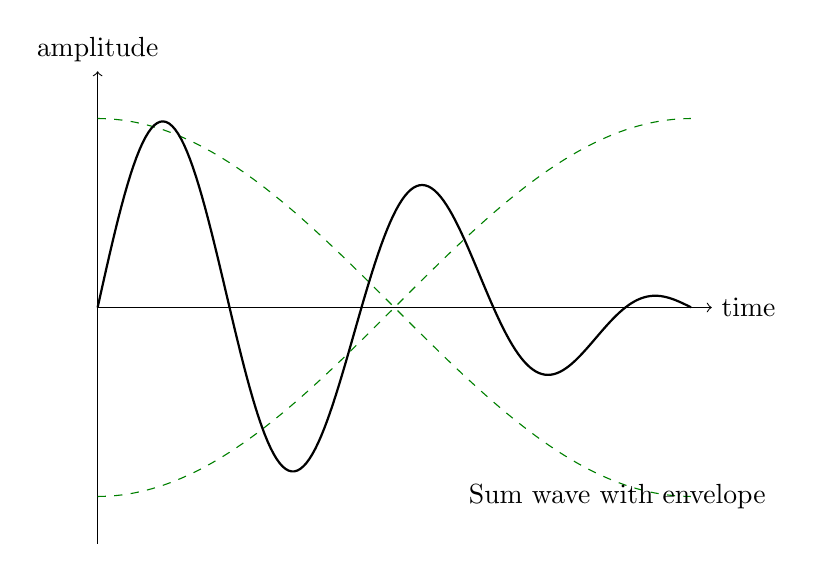
\begin{tikzpicture}[scale=1.2]
\draw[->] (0,0) -- (6.5,0) node[right] {time};
\draw[->] (0,-2.5) -- (0,2.5) node[above] {amplitude};
% Envelope (cosine term)
\draw[green!50!black, dashed, domain=0:6.28, samples=100] plot (\x, {2*cos(0.5*\x r)});
\draw[green!50!black, dashed, domain=0:6.28, samples=100] plot (\x, {-2*cos(0.5*\x r)});
% Sum wave
\draw[thick, domain=0:6.28, samples=200] plot (\x, {2*sin(2.25*\x r)*cos(0.25*\x r)});
\node at (5.5, -2) {Sum wave with envelope};
\end{tikzpicture}
\end{center}

\section{Simple Frequency Ratios and Consonance}

Harmonic consonance occurs when two frequencies form simple integer ratios. The most consonant intervals are:

\begin{center}
\begin{tabular}{llc}
\toprule
Interval & Frequency Ratio & Cents \\
\midrule
Unison & $1:1$ & 0 \\
Octave & $2:1$ & 1200 \\
Perfect Fifth & $3:2$ & 701.96 \\
Perfect Fourth & $4:3$ & 498.04 \\
Major Third & $5:4$ & 386.31 \\
Minor Third & $6:5$ & 315.64 \\
\bottomrule
\end{tabular}
\end{center}

\subsection{Why Simple Ratios Sound Consonant}

When $f_1 : f_2 = m : n$ with small integers $m, n$, the combined waveform repeats after a short period $T = n/f_1 = m/f_2$. The brain perceives this rapid periodicity as stability or consonance. In contrast, irrational ratios produce long or infinite repetition periods, perceived as dissonance.

\subsection{Interference of a 2:1 Ratio (Octave)}

\begin{center}
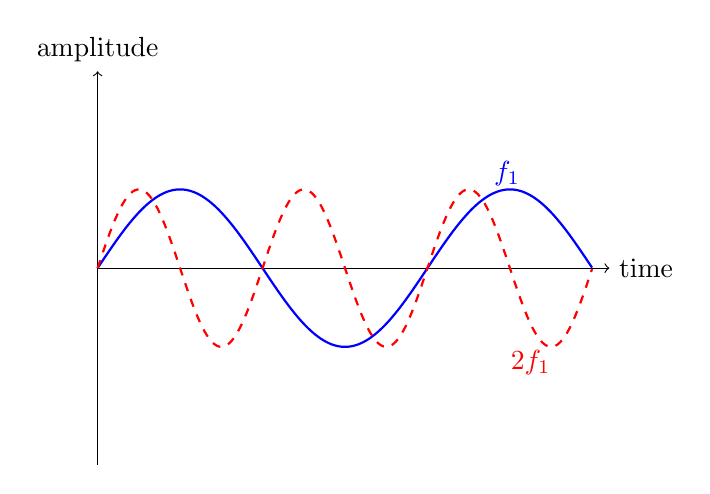
\begin{tikzpicture}[scale=1]
\draw[->] (0,0) -- (6.5,0) node[right] {time};
\draw[->] (0,-2.5) -- (0,2.5) node[above] {amplitude};
\draw[blue, thick, domain=0:6.28, samples=200] plot (\x, {sin(1.5*\x r)});
\draw[red, thick, dashed, domain=0:6.28, samples=200] plot (\x, {sin(3*\x r)});
\node[blue] at (5.2, 1.2) {$f_1$};
\node[red] at (5.5, -1.2) {$2f_1$};
\end{tikzpicture}
\end{center}

Every peak of the lower frequency aligns with every other peak of the higher frequency, creating a stable periodic pattern.

\subsection{Interference of a Complex Ratio}

\begin{center}
\begin{tikzpicture}[scale=1]
\draw[->] (0,0) -- (6.5,0) node[right] {time};
\draw[->] (0,-2.5) -- (0,2.5) node[above] {amplitude};
\draw[blue, thick, domain=0:6.28, samples=200] plot (\x, {sin(1.5*\x r)});
\draw[red, thick, dashed, domain=0:6.28, samples=200] plot (\x, {sin(1.5*\x/1.7 r)});
\node[blue] at (5.2, 1.2) {$f_1$};
\node[red] at (5.5, -1.2) {$\approx 0.588f_1$};
\end{tikzpicture}
\end{center}

The irregular alignment of peaks produces an aperiodic interference pattern, which the auditory system interprets as dissonance or tension.

\section{Fourier Series and Timbre}

Real instruments do not produce pure sine waves. Instead, they produce complex periodic waveforms that can be decomposed into a sum of sinusoids via the Fourier series:

\begin{equation}
    g(t) = \sum_{n=1}^{\infty} a_n \sin(2\pi n f_0 t) + b_n \cos(2\pi n f_0 t),
    \label{eq:fourier}
\end{equation}

where $f_0$ is the fundamental frequency and the coefficients $a_n, b_n$ determine the relative strength of each harmonic. The set of harmonics is called the \emph{harmonic series}.

\begin{center}
\begin{tikzpicture}[scale=1.2]
\draw[->] (0,0) -- (6.5,0) node[right] {time};
\draw[->] (0,-2.5) -- (0,2.5) node[above] {amplitude};
% Sum of first 3 harmonics to approximate a sawtooth
\draw[thick, domain=0:6.28, samples=200] plot (\x, {sin(\x r) + 0.5*sin(2*\x r) + 0.33*sin(3*\x r)});
\node at (4, -2.2) {Sum of first 3 harmonics};
\end{tikzpicture}
\end{center}

Each instrument has a characteristic \emph{timbre} determined by the relative amplitudes of its harmonics. For example:
\begin{itemize}
    \item A flute has mostly the fundamental with weak upper harmonics.
    \item A violin has strong odd and even harmonics giving a rich sound.
    \item A clarinet emphasizes odd-numbered harmonics.
\end{itemize}

The Fourier perspective reveals that the distinction between ``tone'' and ``noise'' is one of periodicity: periodic waveforms produce pitched sounds, while aperiodic waveforms (with continuous Fourier spectra) produce noise.

\section{Tuning Systems}

\subsection{Just Intonation}

Just intonation uses pure integer ratios for all intervals. For a scale based on a fundamental $f_0$, the frequencies are:

\begin{equation}
    f_n = f_0 \cdot \frac{p_n}{q_n}, \quad p_n, q_n \in \mathbb{N}.
\end{equation}

The C major scale in just intonation (relative to C):

\begin{center}
\begin{tabular}{llrl}
\toprule
Note & Ratio to C & Frequency (Hz) & Cents from C \\
\midrule
C  & $1:1$   & 261.63 & 0 \\
D  & $9:8$   & 294.33 & 203.91 \\
E  & $5:4$   & 327.03 & 386.31 \\
F  & $4:3$   & 348.83 & 498.04 \\
G  & $3:2$   & 392.44 & 701.96 \\
A  & $5:3$   & 436.05 & 884.36 \\
B  & $15:8$  & 490.55 & 1088.27 \\
C' & $2:1$   & 523.25 & 1200.00 \\
\bottomrule
\end{tabular}
\end{center}

A limitation of just intonation is that intervals are only pure in one key; modulating to another key introduces wolf intervals.

\subsection{Equal Temperament}

Equal temperament divides the octave into 12 logarithmically equal semitones:

\begin{equation}
    f_{n} = f_0 \cdot 2^{n/12}.
\end{equation}

This allows free modulation between keys at the cost of slightly impure intervals (except the octave). The error in cents compared to just intonation for the perfect fifth is only about 2 cents, which is below the just-noticeable difference for most listeners.

\begin{center}
\begin{tikzpicture}[scale=1]
\draw[->] (0,0) -- (7,0) node[right] {note};
\draw[->] (0,0) -- (0,4) node[above] {frequency (Hz)};
\foreach \x/\label in {0/C, 1/C\#, 2/D, 3/D\#, 4/E, 5/F, 6/F\#, 7/G, 8/G\#, 9/A, 10/A\#, 11/B, 12/C'}
  \draw (\x*0.5, 0.1) -- (\x*0.5, -0.1) node[below, scale=0.7] {\label};
\draw[thick, domain=0:6, samples=200] plot (\x, {261.63*pow(2, \x/12)/100});
\node at (5, 3.5) {$f(n) = f_0 \cdot 2^{n/12}$};
\end{tikzpicture}
\end{center}

\section{Conclusion}

Wave interference provides a mathematical explanation for musical harmony. Simple frequency ratios produce periodic alignment of wave peaks, which the brain interprets as consonance. The beat frequency phenomenon arises naturally from the sum-to-product identity. Fourier analysis reveals that timbre is a consequence of harmonic content, and the choice of tuning system involves a tradeoff between pure intervals and harmonic flexibility across keys.

These results illustrate a deeper principle: mathematical structure in the physical world shapes human aesthetic perception, and the language of waves and frequencies provides a unifying framework for understanding music.

\section*{References}

\begin{enumerate}
    \item Helmholtz, H. (1954). \emph{On the Sensations of Tone}. Dover Publications.
    \item Benson, D. (2006). \emph{Music: A Mathematical Offering}. Cambridge University Press.
    \item Feynman, R. (1964). \emph{The Feynman Lectures on Physics, Vol. I}. Addison-Wesley.
    \item Harkleroad, L. (2006). \emph{The Math Behind the Music}. Cambridge University Press.
    \item Sethares, W. A. (2005). \emph{Tuning, Timbre, Spectrum, Scale}. Springer.
\end{enumerate}

\end{document}
